\documentclass[11pt,titlepage]{article}
\usepackage{geometry}                % See geometry.pdf to learn the layout options. There are lots.
\geometry{letterpaper}                   % ... or a4paper or a5paper or ... 
%\geometry{landscape}                % Activate for for rotated page geometry
%\usepackage[parfill]{parskip}    % Activate to begin paragraphs with an empty line rather than an indent
\usepackage{graphicx}
\usepackage{amssymb}
\usepackage{epstopdf}
\usepackage{url}
\usepackage{hyperref}
\DeclareGraphicsRule{.tif}{png}{.png}{`convert #1 `dirname #1`/`basename #1 .tif`.png}

\title{Microscope Simulator 2.0.0 User's Guide}
\author{Cory Quammen}
%\date{}                                           % Activate to display a given date or no date

\begin{document}
\maketitle
\tableofcontents

\pagebreak

\section{Introduction}

The Microscope Simulator is a program for simulating the imaging process of various microscopes. Currently, simulation of fluorescence microscopes is supported through the FluoroSim module. This modules enables you to see what a geometric model of specimen would look like in a fluorescence microscope under different imaging conditions. Graphics acceleration hardware allows real time generation of simulated microscope images while you interact with specimen models.

The Microscope Simulator serves as a visual problem-solving environment with several applications:

\begin{itemize}

\item building scientist intuition about artifacts in the imaging process by presenting the expected image from a given geometric model

\item evaluating whether a particular microscope can be used to distinguish among hypotheses in an experiment

\item checking the validity of a specimen model by comparing simulated images to experimental images from the lab

\item refining a sub-resolution estimates of a specimen model's shape by automated optimization routines

\end{itemize}

The Microscope Simulator has been designed in close collaboration with biologists to ensure the most useful features are implemented. If you have requests for features, please contact  \href{mailto:cquammen@cs.unc.edu}{Cory Quammen $\langle$cquammen@cs.unc.edu$\rangle$}.


\subsection{System Requirements}

The Microscope Simulator requires Windows XP, Windows 7, or Macintosh OS X 10.5 or higher. A recent graphics card is recommended. We have tested the Microscope Simulator on NVIDIA GeForce 8000 series graphics cards including the GeForce 8800 GTX and Quadro FX 580. More recent NVIDIA graphics cards should also be supported. The Microscope Simulator may work with ATI graphics cards, but we have not tested it on any. The Microscope Simulator will check the capabilities of your graphics card the first time it starts and will warn you if your graphics card is not compatible.

Your system should have at least 100 MB of hard drive space free to install the program. At least 512 MB of RAM is required, but 2 GB is recommended.

\subsection{Acknowledgements}

The Microscope Simulator is developed and maintained by the \href{http://www.cismm.org}{Center for Computer Integrated Systems for Microscopy and Manipulation}, a \href{http://www.nibib.nih.gov/}{National Institute of Biomedical Imaging and Bioengineering Resource}, award number P41-EB002025.

\section{Installation}

Installation of the Microscope Simulator is similar to installation of any other program.

\subsection{Getting the software}

To obtain the latest installer for the Microscope Simulator, visit \url{http://www.cismm.org/downloads}. Source code for the simulator is also available there.

\subsection{Windows installation}

Double-click the setup program named \textbf{MicroscopeSimulator-2.0.0-win32.exe}. On the first screen, click \emph{Next}. Please read the program license. If you agree to the terms of the license, click \emph{I Agree}. On the next screen, choose where you want to install the program. The default directory is the most-used option. Click \emph{Next}. You may optionally choose a different location in the Start Menu. By default, it will be placed in the CISMM folder. Click \emph{Install}.

\subsection{Mac installation}

Double-click the Macintosh disk image named \textbf{MicroscopeSimulator-2.0.0-darwin.dmg}. An installer program will launch and ask you to agree to the terms of the license. If you agree, a disk image named \textbf{MicroscopeSimulator-2.0.0-Darwin} will appear on your desktop and a new Finder window will open.

To install the program in your Applications directory on your computer's hard drive, drag the Microscope Simulator 2.0.0 application to either the Applications alias in the Finder window that just appeared or drag it directly to your Applications directory.

\subsection{Running the program}

\subsubsection{Windows}

You can launch the Microscope Simulator program from the Start menu. If you chose the default installation location and menu folder, select \emph{Start} $\rightarrow$ \emph{All Programs} $\rightarrow$ \emph{Microscope Simulator 2.0.0} $\rightarrow$ \emph{Microscope Simulator 2.0.0}.

\subsubsection{Macintosh}

If you installed the application in the Applications directory on your hard drive, double-click the program \emph{Microscope Simulator 2.0.0}.

\subsubsection{Running the program for the first time}

When you run the Microscope Simulator for the first time, it will run some tests to determine the capabilities of your graphics card. These tests may take a few minutes. Some graphics cards capabilities are required for the program to run while others are optional and enable certain simulation features. If the optional capabilities are not present, then those simulation features will not be enabled. Currently, the only optional graphics card feature enables the generation and addition of pseudo-random Gaussian noise to simulated fluorescence images. If that feature is not available on your graphics card, the control panel section for noise will be disabled.

After the graphics card tests run, the Microscope Simulator will ask for you to choose a data directory where it can store data files. This version of the program stores one small file called \emph{PSFList.xml} which contains the list of point-spread functions defined within the program.

\section{Getting to know the Microscope Simulator}

This section gives you a tour of the many features in the Microscope Simulator.

\subsection{Program Window}

The program window, shown in Figure \ref{fig:ProgramWindow}, consists of several panels. A standard menu bar appears at the top of the window (Windows) or in the system menu bar. Below the menu bar is the \emph{Simulator Control Panel} where settings for the microscopes can be edited. The large panel in the center of the window showing a blue color gradient and grid of white lines is the \emph{Model Display Panel} where specimen models are displayed. Rotating, translating, and scaling models interactively with the mouse also takes place in this window. A row of icons above the \emph{Model Display Panel} controls how specimen models appear and whether simulation results are superimposed with the models. The \emph{Model Settings Control Panel} on the right consists of two parts; the \emph{Model Object List} at the top displays a list of models in the simulation, and the \emph{Model Object Properties Panel} at the bottom displays a list of model properties that can typically be edited. Each of these panels is described in more detail below.

\begin{figure}[htbp] %  figure placement: here, top, bottom, or page
   \centering
   \includegraphics[width=1\linewidth]{images/ProgramWindow-small} 
   \caption{The program window after startup.}
   \label{fig:ProgramWindow}
\end{figure}

\subsection{Menu Bar}

The menu bar in the Microscope Simulator contains five menus that provide commands useful to creating new simulations, adding specimen models to a simulation, saving simulations, and loading saved simulations, among other actions. Each menu is described in more detail below.

\subsubsection{File Menu}

The \emph{File Menu} features typical options for creating and saving simulations:

\begin{description}
  \item[New Simulation] \hfill \\
  Creates a new simulation with default settings.

  \item[Open Simulation...] \hfill \\
  Opens a saved simulation file.

  \item[Save Simulation] \hfill \\
   Saves a simulation's settings to a file. This includes the settings of each microscope simulator, the objects in the scene and their settings, and everything else required to recreate the simulation. If the simulation has not been saved previously, you will be asked to provide a name and location for the file.
   
  \item[Save Simulation As...] \hfill \\
  Does the same thing as the \emph{Save Simulation} menu item, but allows you to save the simulation to another file name.
  
  \item[Exit] \hfill \\
  Exits the program. \textbf{Macintosh users:} The \emph{Quit} menu item appears under the \emph{MicroscopeSimulator} menu instead of the \emph{File} menu.

\end{description}

\subsubsection{Edit Menu}

The \emph{Edit Menu} contains functions common to many programs.

\begin{description}

  \item[Cut] \hfill \\
  \emph{Currently not implemented}
  
  \item[Copy] \hfill \\
  \emph{Currently not implemented}
  
  \item[Paste] \hfill \\
  \emph{Currently not implemented}

\end{description}

\subsubsection{Model Menu}

The \emph{Model Menu} has options for adding and removing geometric models to the simulation. Every model in this menu has parameters that controls its shape. Models are placed at the center of the simulation domain.

\begin{description}

  \item[Add Cylinder] \hfill \\
  Adds a model of a cylinder to the simulation. The ends of the model are capped with flat ends. The length and radius of the tube can be changed.
  
  \item[Add Hollow Cylinder] \hfill \\
  Adds a model of a cylinder with a hollow center to the simulation. Like the cylinder model, the length and outer radius of the tube can be changed. A separate parameter controls the thickness of the tube walls where thickness is defined as the difference between the diameter of the outer and inner cylinder walls.

  \item[Add Disk] \hfill \\
  Adds a model of a planar disk to the simulation. The disk is defined by its center and a radius.

  \item[Add Flexible Tube] \hfill \\
  Adds a model of tube to the simulation. The tube is defined by several control points and a radius. The number of control points can be changed, and each control point can be specified independently.
  
  \item[Add Plane] \hfill \\
  Adds a simple bounded planar model to the simulation. The plane is defined by its width and height.
  
  \item[Add Point Ring] \hfill \\
  Adds a set of an arbitrary number of points to the simulation. The points are restricted to lie in a circle of a given radius. These positions are treated as mathematical points in the simulator, so they are suitable for simulating very small objects such as nanometer-sized particles. No geometry is involved, but the points are represented by small spheres in the \emph{Model Object Window} so that they can be seen easily.
  
  \item[Add Point Set] \hfill \\
  Adds a set of an arbitrary number of points to the simulation. This model is the same as the point ring, but the points are not restricted to lie in a circle. The location of each point can be set independently.
  
  \item[Add Sphere] \hfill \\
  Adds a sphere model to the simulation. The radius of the sphere can be changed.

  \item[Add Torus] \hfill \\
  Adds a torus to the simulation. The radius of the torus and the radius of the cross-section can be adjusted independently.

\end{description}

\subsubsection{Import Menu}

\begin{description}

  \item[Import Image Data...] \hfill \\
  Imports an image file. Single TIFF (2D and 3D) and LSM (Zeiss) files can be imported. You will typically use this when importing an image file to which models should be fit using FluoroSim.
  
  \item[Import Geometry File...] \hfill \\
  Imports geometry from a file. Supported files include:
  
  \begin{itemize}
  \item VTK Files (*.vtk)
  \item VTK Poly Data XML Files (*.vtp)
  \item OBJ Files (*.obj)
  \item PLY Files (*.ply)
  \end{itemize}

\end{description}

\subsubsection{Window Menu}

\begin{description}

  \item[About] \hfill \\
  Shows a window with information about the Microscope Simulator program. \textbf{Macintosh users:} The \emph{About Microscope Simulator} menu item appears under the \emph{Microscope Simulator} menu instead of the \emph{Window} menu. 

  \item[Show Simulator Control Panel] \hfill \\
  Shows/hides the \emph{Simulator Control Panel}. If you close the \emph{Simulator Control Panel}, you can show it again with this menu item.
  
  \item[Show Model Settings Control Panel] \hfill \\
    Shows/hides the \emph{Model Settings Control Panel}. If you close the \emph{Model Settings Control Panel}, you can show it again with this menu item.
  
  \item[Show Fluorescence Window] \hfill \\
  Shows/hides a separate panel that displays the fluorescence images simulated by FluoroSim.
  
  \item[Show Errors] \hfill \\
  Displays a window listing any errors in the program.
  
  \item[Preferences] \hfill \\
  Displays the \emph{Preferences Window} (see Section \ref{sec:PreferencesWindow}).

\end{description}

\begin{figure}[htbp] %  figure placement: here, top, bottom, or page
   \centering
   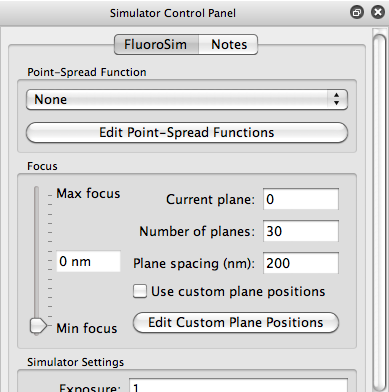
\includegraphics[width=3in]{images/SimulatorControlPanel} 
   \caption{The \emph{Simulator Control Panel} with the \emph{FluoroSim Tab} selected.}
   \label{fig:SimulatorControlPanel}
\end{figure}

\subsection{Simulator Control Panel}

This control panel has two tabs. The \emph{FluoroSim Tab} contains controls for fluorescence simulation. More details on these controls are available in the FluoroSim section of this manual (Section \ref{sec:FluoroSim}). The \emph{Notes Tab} contains a text editor where notes about the current simulation may be written. These notes will be saved in the simulation file and will be loaded when the simulation file is loaded.

\subsection{Model Display Panel}

The \emph{Model Display Panel} is where the 3D specimen models in the simulation are displayed. Output from the Microscope Simulator modules can also be displayed in this window. Such output include fluorophores generated by FluoroSim and fluorescence images superimposed in among the specimen models.

\subsection{Visualization Buttons}

\begin{figure}[htbp] %  figure placement: here, top, bottom, or page
   \centering
   
\includegraphics[width=4in]{images/VisualizationIcons} 
   \caption{The visualization icons.}
   \label{fig:VisualizationIcons}
\end{figure}

A row of visualization icons provide various controls related to what is shown in the \emph{Model Display Panel} (see Figure \ref{fig:VisualizationIcons}). The functions represented by the icons are described from left to right below:

\subsubsection{Utility Buttons}

\begin{description}

  \item[Save Image] \hfill \\
  Save the image currently displayed in the \emph{Model Object Panel}.
  
  \item[Reset Camera] \hfill \\
  Reset the scene to the default view.
  
\end{description}

\subsubsection{Visualization Buttons}

Just one of the following visualization modes can be enabled at a time:

\begin{description}

  \item[View Model Only] \hfill \\
  Displays specimen models only.

  \item[View Fluorophore Sampling] \hfill \\
  Displays fluorophores from models in the scene as small spheres.

%  \item[View Models with AFM Scan] \hfill \\
%  Displays both the specimen models and the simulated AFM surface scan.

  %\item[View AFM Scan Only] \hfill \\
  %Displays the simulated AFM surface scan only.
  
  %\item[View Models with Fluorescence Comparison] \hfill \\
  %Displays comparison of experimental and simulated fluorescence image stacks with the models visible. See the section on processing simulated stacks for more details on the comparison visualization.
  
  %\item[View Fluorescence Comparison Only] \hfill \\
  %Display comparison of experimental and simulated fluorescence image stacks without the models visible. See the section on processing simulated stacks for more details on the comparison visualization.
  
\end{description}
  
\subsubsection{References Axes Button}

Enables/disables display of coordinate axes in the \emph{Model View Panel}. The location of the coordinate axes can be moved to an arbitrary location in the \emph{Model View Panel} display by clicking on the axes and dragging them.
  
\subsubsection{Interaction Modes Button}
  
One of the following interaction modes can be enabled at a time.

\begin{description}

  \item[Move Camera] \hfill \\
  Enables manipulation of the camera in the Model View Panel via mouse manipulation. You can change the view of the specimen models by rotating, translating, and zooming in on the scene. Clicking and dragging while holding different mouse buttons causes different camera motions:

\begin{itemize}
\item \textbf{Left mouse button} - rotates the scene
\item \textbf{Middle mouse button} - translates the scene
\item \textbf{Right mouse button} - zooms in on the scene
\end{itemize}

  \item[Move Objects] \hfill \\
  Enables manipulation of individual specimen model objects via mouse manipulation. Clicking on the desired model object and dragging while holding one of the mouse buttons produces the following transformations:
  
\begin{itemize}
\item \textbf{Left mouse button} - rotates the selected model object
\item \textbf{Middle mouse button} - translates the selected model object
\item \textbf{Right mouse button} - in most cases, scales the size of the model object
\end{itemize}

\end{description}

\subsection{Model Object List}

The model object list appears in the upper right of the program window. All model objects in the simulation are listed here. When you click on a model object in the list, properties for that model object appear in the Model Object Properties Panel. Right-clicking on a model object brings up a context menu that provides several options:

\begin{description}

  \item[Focus on Object] \hfill \\
  Changes the camera view to center on this model object and zoom in on it so that it nearly fills the Model Object View Panel.
  
  \item[Export Geometry] \hfill \\
  Exports the model object geometry as a VTK Legacy file (*.vtk), VTK Poly Data XML file (*.vtp), PLY file (*.ply), or BYU file (*.byu).
  
  \item[Delete Model Object] \hfill \\
  Deletes this model object.

\end{description}

\begin{figure}[htbp] %  figure placement: here, top, bottom, or page
   \centering
   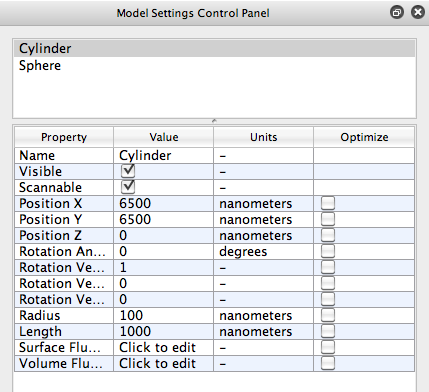
\includegraphics[width=3in]{images/ModelObjectProperties} 
   \caption{The \emph{Model Settings Control Panel}. The \emph{Model Object List} (top section) shows all the specimen models in the simulation. The \emph{Model Object Properties List} (bottom section) contains an editable list of the selected model object's properties.}
   \label{fig:example}
\end{figure}

\subsection{Model Object Properties Panel}

\subsubsection{The Properties Table}

The \emph{Model Object Properties Panel} has four columns showing the properties of the model object selected in the \emph{Model Object List}. Each property is displayed as a row in the table. Most model object properties can be changed in this panel, but some are there to display information about the model object (the size in voxels of an \emph{Image Model Object}, for example).

The \emph{Property} column lists the name of the property. Property names cannot be edited. The \emph{Value} column lists the value of the property. To change the value, click on the table cell. Clicking on a property with a checkbox will toggle the checkbox. Clicking once on a property with a numerical value will select the cell while clicking it twice will highlight the value; in either case, typing a numerical value and pressing the return key will change the property value. The \emph{Units} column shows the units of the parameter and cannot be edited. Unitless properties are denoted with a dash (``-''). The \emph{Optimize} column contains checkboxes to designate which property should be optimized using FluoroSim's model fitting routines (see Section \ref{sec:ModelFittingToFluorescenceImages}).

\subsubsection{Common Model Object Properties}

A few properties common to almost all model objects are listed here:

\begin{description}

  \item[Name] \hfill \\
  A name for the model object.
  
  \item[Visible] \hfill \\
  Controls whether the model object is visible in the scene or not.

  \item[Scannable] \hfill \\
  Controls whether the model object is included when calculating a simulated AFM scan.

  \item[Position X] \hfill \\
   X-component of the model object position.

  \item[Position Y] \hfill \\
  Y-component of the model object position.

  \item[Position Z] \hfill \\
  Z-component of the model object position.
  
  \item[Rotation Angle] \hfill \\
  Angle of rotation in rotation about the vector defined by the next three parameters.
  
  \item[Rotation Vector X] \hfill \\
  X-component of the vector about which the model is rotated.
  
  \item[Rotation Vector Y] \hfill \\
  Y-component of the vector about which the model is rotated.
  
  \item[Rotation Vector Z] \hfill \\
  Z-component of the vector about which the model is rotated.
  
  \item[Surface Fluorophore Model] \hfill \\
  A fluorophore model that samples the surface of the specimen model geometry (see Section \ref{sec:FluorophoreModels}).
  
  \item[Volume Fluorophore Model] \hfill \\
  A fluorophore model that samples the volume defined by boundaries of the specimen model geometry (see Section \ref{sec:FluorophoreModels}).

\end{description}

\subsection{Preferences Window}
\label{sec:PreferencesWindow}

\begin{figure}[htbp] %  figure placement: here, top, bottom, or page
   \centering
   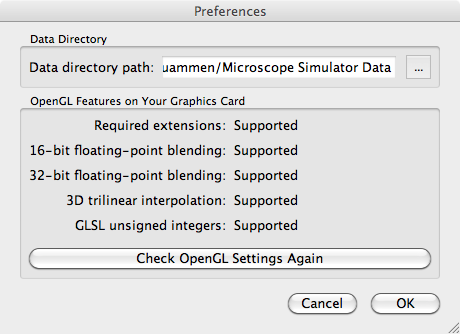
\includegraphics[width=4in]{images/PreferencesWindow} 
   \caption{The Preferences window.}
   \label{fig:PreferencesWindow}
\end{figure}

The \emph{Preferences Window} (Figure \ref{fig:PreferencesWindow}) lets you specify a directory where the Microscope Simulator can store data files. This directory was set the first time the program ran, but it can be changed by clicking on the button to the right of the directory.

The required and optional graphics card capabilities are also listed in the \emph{Preferences Window}. If you install the Microscope Simulator and later upgrade your graphics card, you can check the capabilities of the new card by clicking the \emph{Check OpenGL Settings Again} button. This will also enable the advanced capabilities of the Microscope Simulatorthe when you restart the program.

\section{FluoroSim}
\label{sec:FluoroSim}

\subsection{Model Fitting to Fluorescence Images}
\label{sec:ModelFittingToFluorescenceImages}


%\pagebreak

\section{Version History}

\subsection{Version 2.0.0}

\noindent
Changes from previous release:
\begin{itemize}
\item Complete rewrite of the Microscope Simulator program.
\end{itemize}

\noindent
Known issues:
\begin{itemize}
\item Item
\end{itemize}

\end{document}  